\section{Algorithm Development}
In this chapter, we will provide instruction of the computational algorithm development for the generalized Kubo-Anderson model, introduction on how to install and use the developed software to simulate the stochastic behaviour of the interacting systems in an applied magnetic field including appropriate parameters selection, and provide an introduction to the Master equation and associated transition rate matrix construction for in particular the correct nitroxide spin labelled systems. In addition, we will construct proper Hamiltonian for isolated and coupled spin systems and discuss the resulting simulated spectra in the low and high field approximations with various model parameters.
\subsection{Liouville Matrix Inverse Algorithm}\label{algorithmsection}
In order to simulate a lineshape from a system undergoing stochastic relaxation effects as applied to spin dynamics and discussed in previous chapter \ref{chapter1},  one of the major efforts of this work was to develop a generalized algorithm to invert the Liouville matrix given in Eq.\ref{eq:35}. The construction of such a matrix can be described in terms of a two dimensional array where each index has an additional three sub-indices specified by stochastic, electronic and/or nuclear spin states depending on whether NMR or ESR/EPR spectra are being simulated and incorporating specific system interactions (Zeeman, dipolar, quadrupolar, etc). Specifically, the following matrix representation is relevant: 
\begin{equation}\label{eq:liv2d}
\mathcal{L}_{i,j}=\mathcal{L}_{a,m_0,m_1;b,m_0',m_1'}  
\end{equation}  
Where $i\rightarrow a,m_0,m_1$ and $j\rightarrow b,m_0',m_1'$. This is a straightforward index mapping but computationally there are two approaches that are feasible. In the first approach, matrix in Eq.\ref{eq:liv2d} is considered to be strictly two dimensional and each index should be worked out manually. This task is acceptable when working with isolated spin systems (see example in \ref{blumeinitialmodel} and \ref{zeemansection}). When dealing with non-isolated spin systems one can expect to derive more then 1000 matrix elements manually. This task rapidly becomes inefficient and time-consuming. In the second approach, the Liouville matrix sub-indices are flattened into separate dimensions, the lengths of which are specified according to the quantum and stochastic states of the simulated system:  
\begin{equation}\label{eq:54}
\mathcal{L}_{i,j}=\mathcal{L}_{a,m_0,m_1;b,m_0',m_1'}\rightarrow \mathcal{L}[a][m_0][m_1][b][m_0][m_1]
\end{equation}
The majority of high-level programming languages such as Java, Python or C++ natively support operations with multidimensional arrays meaning that no additional open source or proprietary libraries are required. Multidimensional representation of the Liouville matrix also radically simplifies computation of its elements as the summation is constrained from Eq.\ref{eq:33}. Naive implementation might lead to spurious structural patterns in the lineshape. Computationally, access of the matrix elements of dimensions higher than 2 can be done using a 'page' representation shown on fig.\ref{figure:matlabnd}. Basically, it can be visualized such that each index for higher dimensions is being projected on a separate page with row and column indexes as follows: 
\begin{figure}[h!]
\centering
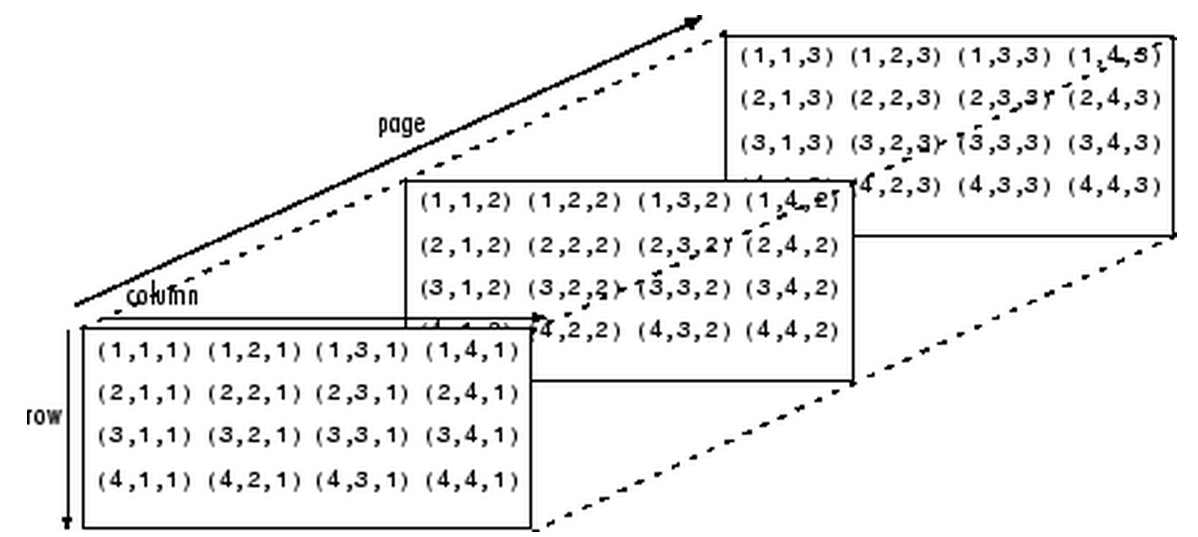
\includegraphics[width=0.7\textwidth]{figures/chap1/mat.png}
\caption{Illustration of 'page' concept of storing and accessing elements of 3-dimensional array $A_{4,4,4}$ or $A[4,4,4]$ depending on syntax familiarity with four elements in each dimension.~\cite{Matlab}}. 
\label{figure:matlabnd}
\end{figure}
For example, the Liouville matrix for an isolated nuclear spin has six dimensions $\Big(\mathcal{L}[a][m_0][m_1][b][m_0][m_1]\Big)$ and when an electron spin interaction is added it expands to overall 10 dimensions specified by four additional sub-indexes $m_{0S},m_{1S},m_{0S}',m_{1S}'$ or $\Big(\mathcal{L}[a][m_{0S}][m_{1S}][m_0],[m_1][b][m_{0S}][m_{1S}][m_0],[m_1]\Big)$. If we assume rows and columns primarily are indexed by stochastic $a$ and $b$ states, then the quantum states are stored on separate 'pages' as shown in fig.\ref{figure:matlabnd}. \\*
In general, when all possible interactions are included the constructed Liouville matrix will be highly sparse. This is true for the slow motion regime and when non-secular Hamiltonian terms are retained as we will show in \ref{blumeinitialmodel} and \ref{zeemansection}. This condition limits us from using standard techniques to invert multidimensional arrays. In the standard approach, each 'page' that is represented as a 2-D array would be inverted using any suitable algebraic approach~\cite{solo}. In our case not all sub-matrixes have non-zero determinant and a errors will occur on compilation. We reshape the N-dimensional array to a square 2-D form and perform inversion. Basically we flattened Eq.\ref{eq:liv2d} and developed a key-value transformation of the N-D array storing information for each set of sub-indexes into a primitive type such as double or string and creating a corresponding hash table.\\*
The example of such index mapping can be demonstrated on a particular case with $a=b=4$, $m_0=m_0'\pm1/2$ and $m_1=m_1'\pm1/2$. Thus transformation from a 6-D array of size $4\times4\times2\times2\times2\times2$ to 2-D $16\times16$ can be described in Table.\ref{table:kysymys}.
\begin{table}[h!]
\begin{center}
    \begin{tabular}{  l  l  l  l l }
    \hline
    $a,m_0,m_1$ &  & Output & Key\\ \hline
    $1,1/2,1/2$ & $\rightarrow$ & 000 & 1 \\ \hline
    $1,-1/2,1/2$ & $\rightarrow$ & 010 & 2  \\ \hline
    $1,1/2,-1/2$ & $\rightarrow$ & 001 & 3 \\ \hline
    $1,-1/2,-1/2$ & $\rightarrow$ & 011  & 4\\ \hline
    $2,1/2,1/2$ & $\rightarrow$ & 100 & 5 \\ \hline
    $2,-1/2,1/2$ & $\rightarrow$ & 110 & 6  \\ \hline
    $2,1/2,-1/2$ & $\rightarrow$ & 101 & 7 \\ \hline
    $2,-1/2,-1/2$ & $\rightarrow$ & 111  & 8\\ \hline
    $3,1/2,1/2$ & $\rightarrow$ & 200 & 9 \\ \hline
    $3,-1/2,1/2$ & $\rightarrow$ & 210 & 10  \\ \hline
    $3,1/2,-1/2$ & $\rightarrow$ & 201 & 11 \\ \hline
    $3,-1/2,-1/2$ & $\rightarrow$ & 211  & 12\\ \hline
    $4,1/2,1/2$ & $\rightarrow$ & 300 & 13 \\ \hline
    $4,-1/2,1/2$ & $\rightarrow$ & 310 & 14  \\ \hline
    $4,1/2,-1/2$ & $\rightarrow$ & 301 & 15 \\ \hline
    $4,-1/2,-1/2$ & $\rightarrow$ & 311  & 16\\ \hline
    \end{tabular}
\end{center}
\caption{Hash table of the Liouville matrix $i$-th index for Java and Python. Array enumeration starts with 0-th element}
\label{table:kysymys}
\end{table}
 The $j$-th index can be encoded similarly to the $i$-th index. There will be no hashing ambiguity based on assumption that no more then $2^{31}-1$ indexes are needed. We can easily re-construct the N-D array from the stored hash table to perform the summation defined in Eq.\ref{eq:33}. Now we can define all the steps of the Liouville matrix assignment and transformation:  
\begin{center}
\begin{enumerate}
\item Assign Liouville multidimensional matrix: $\mathcal{L}[a,m_0,m_1,b,m_0',m_1']$
\item Transform multidimensional matrix into 2-dimensional: $\mathcal{L}[a,m_0,m_1,b,m_0',m_1'] \rightarrow \mathcal{L}'[i,j]$ 
\item Transformed matrix inversion: $\mathcal{L}'[i,j]=\mathcal{L}'[i,j]^{-1}$
\item Transformation of 2-dimensional matrix back to multidimensional: \\ $\mathcal{L}'[i][j]\rightarrow \mathcal{L}[a,m_0,m_1,b,m_0',m_1']$ 
\end{enumerate}   
\end{center}    
Now that we have demonstrated the algorithm we can proceed with a description of the written software.
\section{SpinAl Program}
For software development we have used Java primarily for its compilation speed, garbage collection capabilities and portability ~\cite{hortell}~\cite{javapal}. Multidimensional arrays are represented as an N-dimensional superclass object as part of java.util.Arrays package. Any interaction between objects in Java is valid if their interaction is defined through the methods that are specified for both of them. On the basis of all these considerations we have written SpinAl program in Java. It has a natively simple interface and comes packaged as SpinAl.jar file. It can be launched on any machine with the Java 7+ environment installed. On MacOS and Linux we can either double tap on the jar-file or use the terminal to launch it:
\begin{lstlisting}
$ java -jar SpinAl.jar
\end{lstlisting}
The main menu on Fig.\ref{figure:SpinAl1} appears asking the user to specify the stochastic values $a$ and $b$ as well as frequency range. The following menu on Fig.\ref{figure:SpinAl2} requires the user to enter precise details on the values of fixed and fluctuating magnetic fields based on the Hamiltonian described by Eq.\eqref{eq:blumeham}. Also the transition rate for the stochastic process has to be specified. We expect the stochastic proces to be bijective thus an exception will be thrown if $a\neq b$. 
\begin{figure}[h!]
\centering
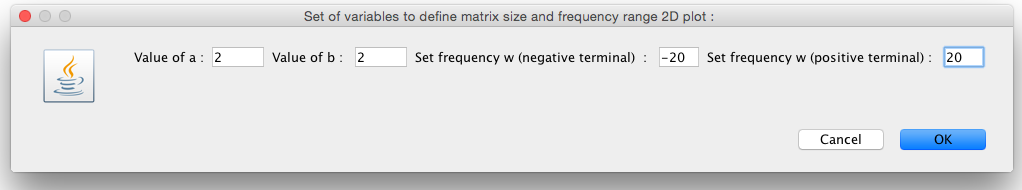
\includegraphics[width=0.8\textwidth]{figures/chap2/spinal1.png}
\caption{Main menu of the SpinAl software with parameters selection for stochastic indexes and frequency range.}
\label{figure:SpinAl1}
\end{figure}
For this specific example we set $a$ and $b$ as 2. The frequency range is $-20\leq\omega\leq 20$ in frequency units. Fixed magnetic field as 4 frequency unitsand fluctuating magnetic field along z-axis with a value of 3 in frequency units. The transition rate value was arbitrarily chosen as 0.01 in frequency units. The meaning of these parameters, the Hamilton derivation and the Liouville matrix population are discussed in section\ref{blumeinitialmodel} 
\begin{figure}[h!]
\centering
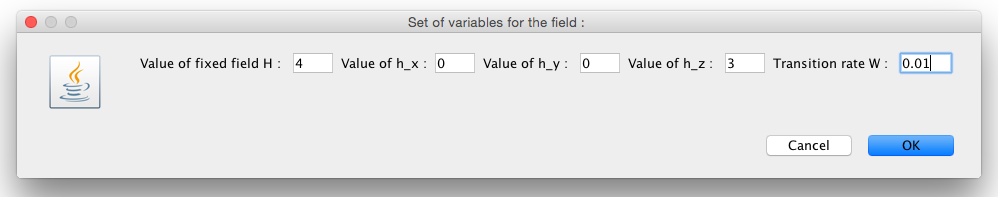
\includegraphics[width=0.8\textwidth]{figures/chap2/spinal2.png}
\caption{Proceeding menu of the SpinAl software with parameters selection for applied and fluctuating magnetic field as well as transition rate $W$.}
\label{figure:SpinAl2}
\end{figure}
\begin{figure}[h!]
\centering
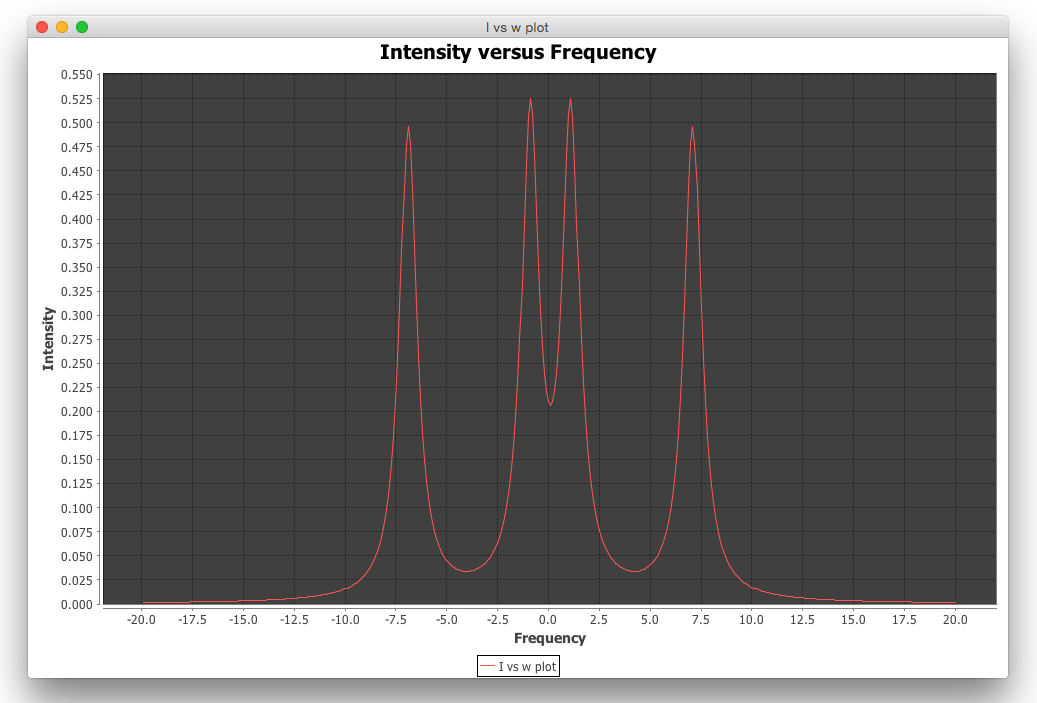
\includegraphics[width=0.8\textwidth]{figures/chap2/spinal3.png}
\caption{Simulated spectrum graph of intensity versus Frequency after all model parameters have been entered.}
\label{figure:SpinAl3}
\end{figure}
The output of the computation is a graph of Intensity versus frequency as shown in Fig.\ref{figure:SpinAl3}.
Currently SpinAl is limited to 2, 6 and 48 stochastic indexes as the transition rate matrix under rotations is developed for these specific cases. We plan to generalize the software in future releases by adding the possibility of creating custom $W$-matrix as well as rotation angles that could be uploaded as text files and parsed by SpinAl. Source code is available at the authors public GitHub repository under open license\cite{nmrgit}.\\
The core algorithm of SpinAl to invert N-D arrays has been separated into a framework available in separate GitHub repository\cite{ndgit}. It supports up to 10-D complex arrays inversion. Maximum size of supported arrays is limited precisely as: \ Array[100][100][10][10][10][10][10][10][10][10].\\*
While working on SpinAl our group was also exploring alternative possibilities to make computation cost-efficient. Thus, we have successfully ported SpinAl to the Python programming language. From benchmarking prospective and garbage handling Java has advantages over Python~\cite{slower}but lacks simplicity in development. Also with the rise of Machine Learning and Deep Learning research for which the majority of relevant frameworks are coded in Python, there are more advanced compilers available that minimize the speed difference between languages. Currently our Python 2.7 written SpinAl does not have a user interface but this will be added in future releases. All program interaction is done through the command line. We have also replaced N-D array inversion by native methods from scientific libraries such as NumPy and SciPy~\cite{SciPy1}~\cite{SciPy2}. Algebraic manipulations on N-Dimensional arrays that are available in NumPy have two different algorithms on reshaping arrays in Fortran-like and C-like manner. Most of the well-known libraries for Magnetic Resonance spectral simulations are written in Fortran and thus using Python wrappers for Fortran code is a viable choice to efficiently use in software projects along with developed program. We have also explored the possibility of using GPU~\cite{gpu} computations on the CUDA platform. Simulated spectra provided reported in this work were obtained from the Python version of SpinAl unless specified otherwise. Python source code is available at GitHub repository as well~\cite{eprgit}\\*
We have also developed numerous tools for proof-of-concept as well as transition rate matrix population in Matlab which are available upon request from Professor Keith Earle Lab. We have also rewritten SpinAl core algorithm in Python however the computational performance was similar to the one written in Java. In a later release C-like N-dimensional array inversion became available in Matlab, however we were not able to reproduce slow motion regime spectra obtained from either Java or Python versions of the code. For computation purposes a machine with Intel 3rd generation Core i7 3630QM processor, 16 GB DDR3 1600GHz memory and equipped with NVIDIA GTX 670 MX graphic processing unit (960 cores) was used.\\* 
\subsection{Transition Rate Matrix}\label{trmsection}
In order to further specify the interacting environment, discussed in section \ref{kuboandersonsection}, we need to determine suitable number of stochastic states $a$ and $b$ that form a two dimensional matrix $W$ known as a transition rate matrix. We began by discussing the transition rate matrix from a probabilistic approach. We have discussed the computational algorithm performance in a previous section \ref{algorithmsection} but have not yet established the relation between 2,6 and 48 stochastic indexes and their significance. One of our goals in this research work was to determine lower bound of discrete states that are necessary to faithfully reproduce an ESR lineshape using concepts derived from information geometry\cite{Earle2009}.\\*
As an example of transition rate matrix construction we will start by introducing a two-state system that can uniformly and randomly transit between its states such as chemical exchange where a nucleus moves reversibly from one environment to another at a constant rate. A probabilistic approach to describe the time evolution of large discrete fluctuating systems is widely used in economics\cite{Weidlich1992}. Let us assume that for the nuclear transition to one state is defined by the rate $\omega_{1\rightarrow2}$ and jump back as $\omega_{2\rightarrow1}$ or simply $\omega_{12}$ and $\omega_{21}$. Corresponding probabilities are $P_{1}(t)$ and $P_{2}(t)$ that the nucleus is either in one or the other state. We make the Markov assumption that the transition rate between states does not depend on the history of the process but rather on the state at specific time $t$ between enclosed time intervals $(t,t+dt)$. Further the probability of a nucleus being in state 1 between $(t,t+dt)$ can be described as following: 
\begin{equation}\label{eq:premaster}
P_{1}(t+dt)=P_{1}(t)[1-\omega_{12}dt]+P_{2}\omega_{21}dt+\mathcal{O}(dt^2)
\end{equation} 
The first term arises from assumption that nucleus does not transition to the second state and second term represents transition back to the state 1 in a given time interval. The last term $\mathcal{O}(dt^2)$ came from assumption that particle could follow a chain from $1\rightarrow 2 \rightarrow 1$. Taking a limit $dt\rightarrow 0$ the result appear to be a simple set of differential equations: 
\begin{equation}\label{eq:masterlol}
\frac{dP_{1}}{dt}=-\omega_{12}P_{1}(t)+\omega_{21}P_{2}(t)
\end{equation}
In general we can write for an arbitrary number of states: 
\begin{equation}\label{eq:master}
\frac{dP_{i}}{dt}=-\sum_{j\neq i}\omega_{i\rightarrow j}P_{i}+\sum_{j\neq i}\omega_{j\rightarrow i}P_{j}
\end{equation}
Eq.\ref{eq:master} is known as the Master Equation. In vector form:   
\begin{equation}\label{eq:matrix}
\frac{d\vec{p}}{dt}=-\vec{W}\vec{p}
\end{equation} 
Where $\vec{p}$ is a column vector with probabilities $p_i$ and $\vec{W}$ is a square transition rate matrix.
Solution of the master equation requires eigenvalue and eigenvector decomposition of the matrix $W$ which can be a difficult task for large stochastic systems. Also note that the diagonal elements of $W$ are defined as:  
\begin{equation}\label{eq:markov3}
-W_{i,i}\equiv\sum_{j,j\neq i}W_{i,j}
\end{equation} 
Accordingly we can construct a two-state system transition matrix as the following:   
\begin{equation}\label{eq:55}
W = \begin{bmatrix}
       -w_{11} & w_{12}  \\[0.3em]
        w_{21} & -w_{22}  
     \end{bmatrix}
\end{equation}
Diagonal elements are defined via Eq.\ref{eq:markov3} and it means that probability leaving the state is equal to the probability of reaching it.
For modelling nitroxide spin labels we need to determine an adequate number of stochastic states to cover all possible orientations. We started by developing a 6 state transition rate matrix. In geometrical three-dimensional representation it is an octahedron. A graph of allowed transitions (adjacency matrix) is given on Fig.\ref{figure:wdiagramm}.     
\begin{figure}[h!]
\begin{center}
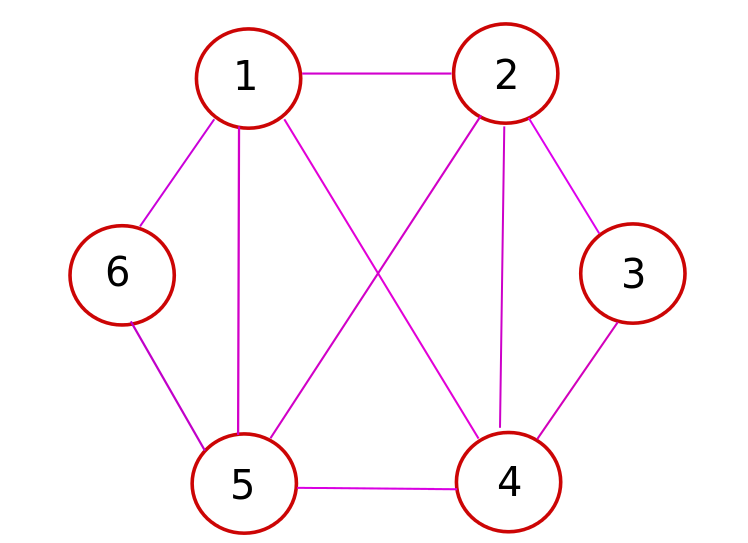
\includegraphics[width=0.7\textwidth]{figures/chap2/wdiagramm.png}
\caption{transition probabilities graph between 6 possible events}
\label{figure:wdiagramm}
\end{center}
\end{figure}
We can precisely define the $W$ matrix based on \ref{figure:wdiagramm} as follows: 
\begin{equation}\label{eq:Wmat1}
W = \begin{bmatrix}
       w_{11} & w_{12} & 0 & w_{14} & 0 & w_{16}  \\[0.3em]
       w_{21} & w_{22} & w_{23} & 0 & w_{25} & 0  \\[0.3em]
       0 & w_{32} & w_{33} & w_{34} & w_{35} & 0  \\[0.3em]
       w_{41} & 0 & w_{43} & w_{44} & w_{45} & 0 \\[0.3em]
       0 & w_{52} & 0 & w_{54} & w_{55} & w_{56} \\[0.3em]
       w_{61} & 0 & w_{63} & 0 & w_{65} & w_{66} 
     \end{bmatrix}
\end{equation}
This matrix is assumed to be symmetric with equal priory probabilities which is not always the case when transition probabilities are not isotropic. As an example of isotropic transition probabilities recall that transformation of the principal axis frame of $g$ or $A$ tensors that are parameterized by Euler angles and one can define unequal a priory probabilities and fast transition as $\vec{R}(0,0,0)\xrightarrow {1\rightarrow 6}\vec{R}(0,0,\pi/2)$. Similarly moderate $\vec{R}(0,0,0)\xrightarrow {1\rightarrow 2}\vec{R}(0,\pi/2,0)$  and slow $\vec{R}(0,0,0)\xrightarrow {1\rightarrow 4}\vec{R}(\pi/2,0,0)$ which imply the re-constructed matrix:   
\begin{equation}\label{eq:Wmat2}
W = \begin{bmatrix}
       0 & m & 0 & s & 0 & f  \\[0.3em]
       m & 0 & s & 0 & f & 0  \\[0.3em]
       0 & s & 0 & f & m & 0  \\[0.3em]
       s & 0 & f & 0 & m & 0 \\[0.3em]
       0 & f & 0 & m & 0 & s \\[0.3em]
       f & 0 & m & 0 & s & 0 
     \end{bmatrix}
\end{equation}
Where $s,m$ and $f$ define three probability transition rates: slow, moderate and fast respectively which affect the details of the line shpae and will be discussed in the next chapter.\\*
For complex interactions we need significantly more then 6 stochastic states. We approach generalization by treating stochastic states as randomly generated points on an N-dimensional hypersphere or simply 4-sphere. This approach is fairly well accepted in algorithm development in robotics on problems in space orientations\cite{robotics}\cite{ershova}. 
In addition to distributing uniformly points on a sphere we also need to take into account its reference frame transformations specified by the $SO(3)$ orthogonal group. For this purpose it is useful to use projective space methods based on quaternions which simplifies the Euler angles calculation compared to Hopf or spherical coordinates. The initial decoration algorithm is straight forward and was developed by Cook\cite{cook}. We pick $\lambda, \Lambda_x, \Lambda_y,\Lambda_z$ from a uniform distribution on $(-1,1)$ and reject points that do not meet the following condition: 
\begin{equation}\label{eq:cook}
\lambda^2+\Lambda_x^2+\Lambda_y^2+\Lambda_z^2\geq1
\end{equation}
In this decoration we obtained 48 stochastic states related rotations by $\pi/2$. The corresponding adjacency matrix has been constructed such that each state has 6 nearest neighbours at distance of $\pi/4$. Euler angles have been reconstructed using equations Eq.\ref{eq:1911}-\ref{eq:194}. For this specific case we assumed equal a priory probabilities and in future work it will be another challenge to determine a transition probability distribution for this case. 
\begin{figure}[h!]
\begin{center}
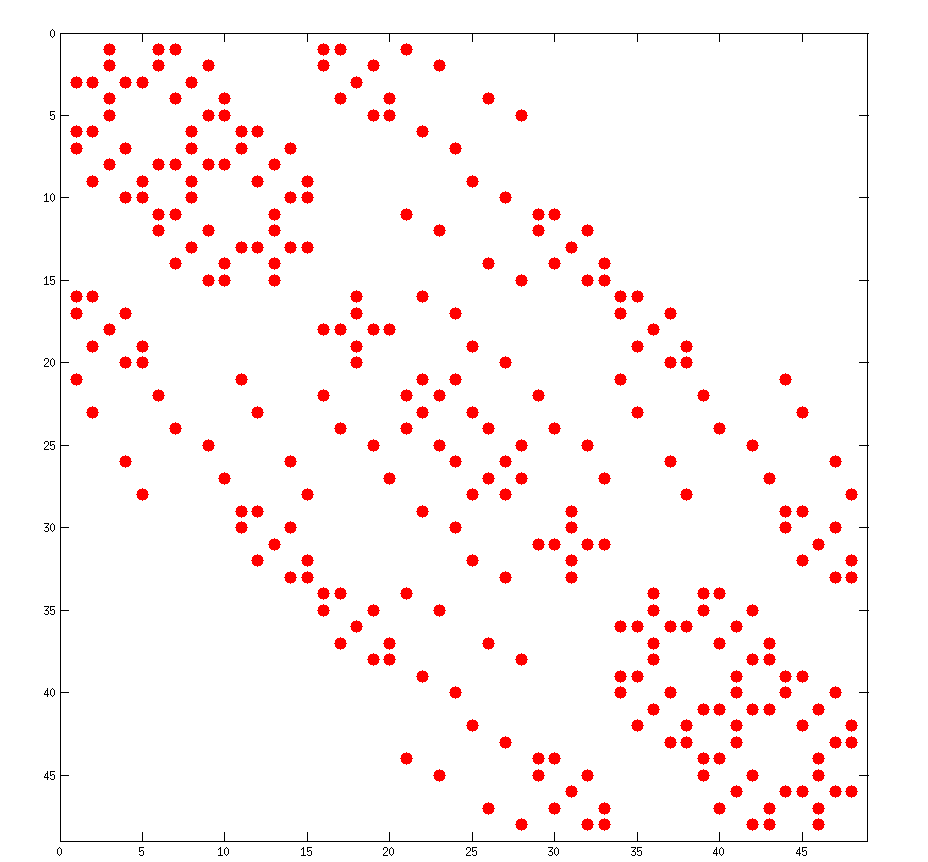
\includegraphics[scale=0.5]{figures/chap2/sparce.png}
\caption{Illustration of allowed transitions between 48 states defined by quaternion representation of rotation points on $S_3$. Allowed transitions are in red.}
\label{figure:blumediag}
\end{center}
\end{figure}  
\clearpage
\subsection{Algorithm Validation}\label{blumeinitialmodel}
To validate algorithm implemeted in SpinAl we have decided to reproduce original absorption spectra of isolated spin-1/2 nucleus in a fixed magnetic field and fluctuating local fields along $x,y$ and $z$ orientations described in original Blume paper~\cite{blume}. In this particular setting $I_0=I_1=1/2$ and transitions are defined between $m_{0}=\pm\frac{1}{2}$ and $m_{1}=\pm\frac{1}{2}$. Transition matrix defined from \ref{eq:55} and equal a priori probabilies assumed between the transitions. As there are two stochastic states $p_a=p_b=1/2$.\\*
Time dependent Hamiltonian that consists of Zeeman interaction term is given as following: 
\begin{equation}\label{eq:58}
\mathcal{H}(t)=B_0I_z+\vec{h}\cdot\hat{I}f(t)
\end{equation}  
Fixed magnetic field $B_0$ by NMR and EPR/ESR convention in this case is set along $z$ axis and fluctuating local field $h(x,y,z)$ can point in any arbitrary direction. Stochastic function $f(t)$ can take two values 1 or -1. In feasible form Eq. \ref{eq:58} can be written as: 
\begin{equation}\label{eq:blumeham}
\mathcal{H}(t)=B_0I_z+f(t)\big[\frac{1}{2}(h_+I_-+h_-I_+)+h_zI_z\big]
\end{equation}     
Where $I_{\pm}$ are rising and lowering nuclear spin operators and $h_{\pm}=h_x\pm h_y$ and $h_z$ defines fluctuating field in associated with spin operators in $x,y,z$ planes. \\*
Dimension of Liouville matrix is $8\times 8$ and its precise and accurate construction from Eq. \ref{eq:35} is presented in Eq.\ref{eq:60}. In the case when local fluctuating fields aligned with the applied field $h_+=h_-=0$ matrix Eq.\ref{eq:60} reduces to banded or sparse matrix with two non-zero diagonals Eq.\ref{eq:61}. Thus $8\times 8$ matrix reduce to four $2\times 2$ and from computational prospective it is possible to take to account only the two middle matrices and invert them separately which is less time consuming. This is not always the case and in EPR and off-diagonal elements can carry important structural information. \\*
Following procedure from Blume \cite{blume} fixed field was set to $B_0=3$ and fluctuating field $h=h_x=h_y=h_z=4$. Results are presented on Fig.\ref{figure:blumediag}. For all (a), (b) and (c) for fast modulation regime line shape is represented by sharp Lorentizan peak centred around Zeeman frequency. At shorter transition rates thus slow relaxation regime case (a) and (b) represent absorption spectra with fluctuating local fields along $x$ and $y$ axis. The peak roughly occurs at $\omega\approx(B_0^2+h^2)^{1/2}$. Additional Broad side peak at  Fig.\ref{figure:blumediag}(a) can be explained as image of electric non-static Gaussian electron field strength distribution. For the case at Fig.\ref{figure:blumediag}(c) fluctuating field along $z$ axis and two lines correspond to each of the two state frequencies defined as $\omega\approx B_0\pm h$. Fig.\ref{figure:blumediag}(c) corresponds to classical example of temperature dependence of NMR and EPR spectrum due to chemical exchange. In all three cases with the increasing of transition rates lines are broadening at some moderate rate and then collapse into one narrowed line as change of stochastic transitions averages out. \\*
Simulated figures at Fig.\ref{figure:blumediag}(c) completely agrees with originally proposed by Blume \cite{blume} and were obtained by manually typing Liouville matrix and performing inversion and summation to obtain absorption spectra and by AI generalized algorithm. Both computational cases converged to one solution which was an indicator of AI validity and robustness.  
As simple example of such system chemical exchange consider two $N$-methyl groups in $N,N'$ - dimethylformamide can exchange their relative bond and reactant chemically and physically remains indistinguishable from the product. Methyl groups are colored in red and black to make process visible.       
\begin{figure}[h!]
\centering
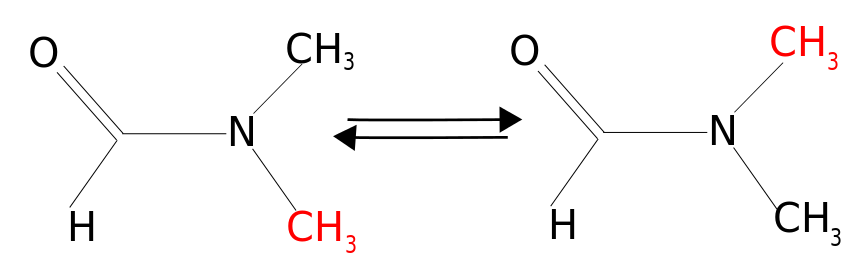
\includegraphics[width=0.7\textwidth]{figures/chap2/methil.png}
\caption{$N,N'$ -
dimethylformamide chemical exchange of methyl groups in active moiety.}
\label{figure:methyl}
\end{figure}
Magnetic environment of $N$-methyl groups will be different after the chemical exchange which leads to the fact that they will have different resonance frequencies before and after the reaction and molecular motion can be treated by Blume stochastic model. Example of the NMR spectra dependence on temperature is given on Fig.\ref{figure:datamet} 
\begin{figure}[h!]
\begin{center}
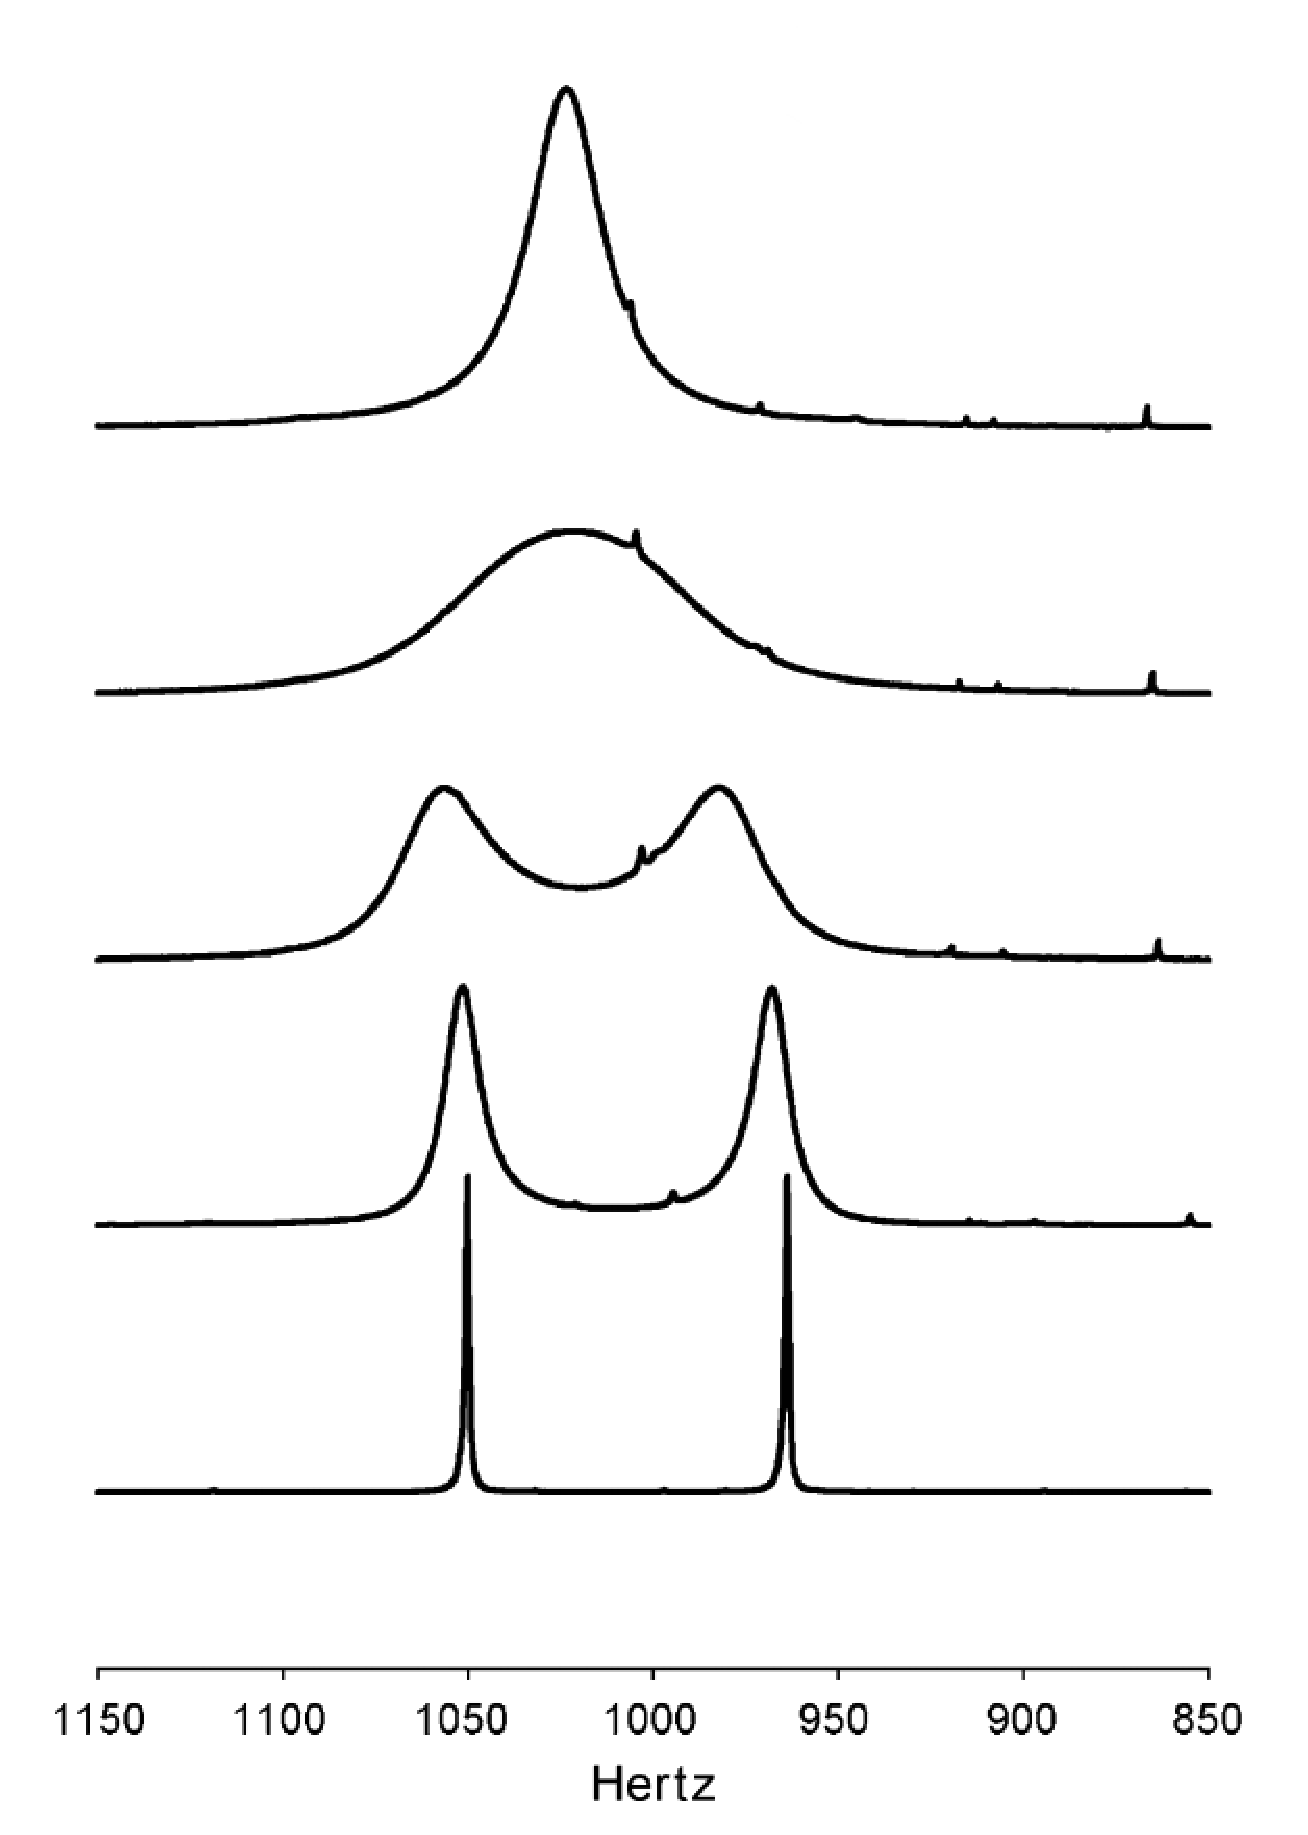
\includegraphics[scale=0.5]{figures/chap2/methyldat.eps}
\caption{"Proton NMR spectra at 300 MHz of the $N$-methyl signals in a
derivative of azapropazone as a function of temperature. The lowest spectrum is at 223 K, and then
at 243, 253, 263, and 273 K"~\cite{Bain200363}}
\label{figure:datamet}
\end{center}
\end{figure}           
        
\clearpage
\begin{landscape}
\begin{equation}\label{eq:60}
\mathcal{L} = \begin{bmatrix}
       p-w_{aa} & -w_{ab} & \frac{1}{2}h_+ & 0 & -\frac{1}{2}h_- & 0 & 0 & 0  \\[0.3em]
       -w_{ba} & p-w_{bb} & 0 & -\frac{1}{2}h_+ & 0 & \frac{1}{2}h_- & 0 & 0  \\[0.3em]
       \frac{1}{2}h_- & 0 & p-w_{aa}-i(B_0+h_z) & -w_{ab} & 0 & 0 & -\frac{1}{2}h_- & 0  \\[0.3em]
       0 & -\frac{1}{2}h_- & -w_{ba} & p-w_{bb}-i(B_0-h_z) & 0 & 0 & 0 & \frac{1}{2}h_-  \\[0.3em]
       -\frac{1}{2}h_+ & 0 & 0 & 0 & p-w_{aa}-i(B_0+h_z) & -w_{ab} & \frac{1}{2}h_+ & 0  \\[0.3em]
       0 & \frac{1}{2}h_+ & 0 & 0 & -w_{ba} & p-w_{bb}+i(B_0-h_z) & 0 & -\frac{1}{2}h_+  \\[0.3em]
       0 & 0 & -\frac{1}{2}h_+ & 0 & \frac{1}{2}h_- & 0 & p-w_{aa} & -w_{ab}  \\[0.3em]
       0 & 0 & 0 & \frac{1}{2}h_+ & 0 & -\frac{1}{2}h_- & -w_{ba} & p-w_{bb} 
     \end{bmatrix}
\end{equation}
\end{landscape} 

\begin{landscape}
\begin{equation}\label{eq:61}
\mathcal{L} = \begin{bmatrix}
       p-w_{aa} & -w_{ab} & 0 & 0 & 0 & 0 & 0 & 0  \\[0.3em]
       -w_{ba} & p-w_{bb} & 0 & 0 & 0 & 0 & 0 & 0  \\[0.3em]
       0 & 0 & p-w_{aa}-i(B_0+h_z) & -w_{ab} & 0 & 0 & 0 & 0  \\[0.3em]
       0 & 0 & -w_{ba} & p-w_{bb}-i(B_0-h_z) & 0 & 0 & 0 & 0  \\[0.3em]
       0 & 0 & 0 & 0 & p-w_{aa}-i(B_0+h_z) & -w_{ab} & 0 & 0  \\[0.3em]
       0 & 0 & 0 & 0 & -w_{ba} & p-w_{bb}+i(B_0-h_z) & 0 & 0  \\[0.3em]
       0 & 0 & 0 & 0 & 0 & 0 & p-w_{aa} & -w_{ab}  \\[0.3em]
       0 & 0 & 0 & 0 & 0 & 0 & -w_{ba} & p-w_{bb} 
     \end{bmatrix}
\end{equation}
\end{landscape} 

\begin{figure}[h!]
\centering
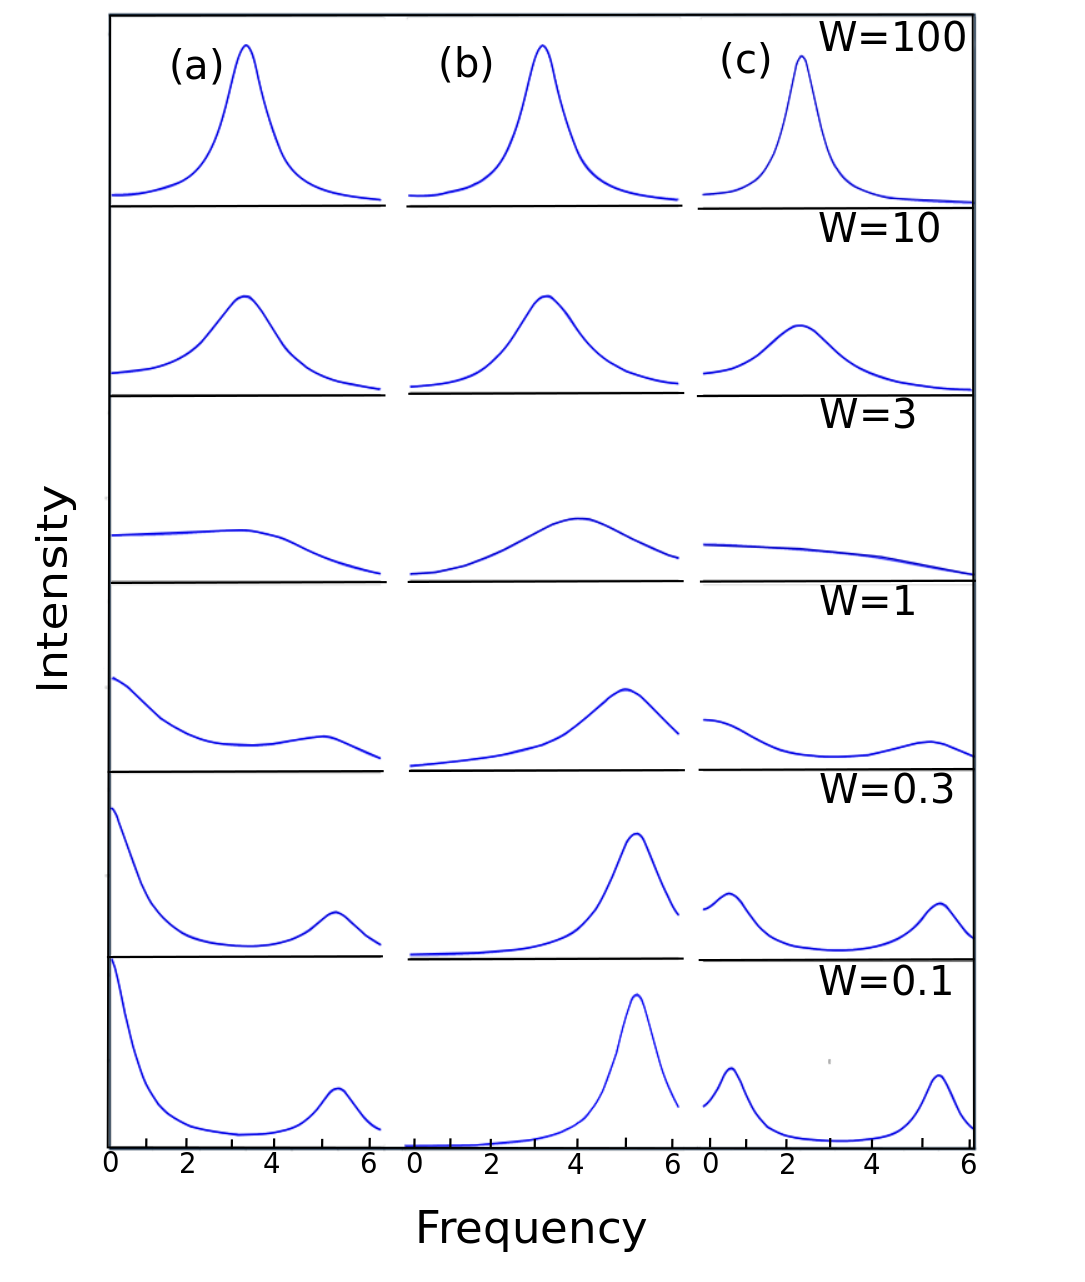
\includegraphics[width=0.7\textwidth]{figures/chap2/blumediag.png}
\caption{Evolution of NMR line shapes with increase of transition rates $W$ for $I=1/2$ nucleus in a fixed magnetic field along $z$ axis and fluctuating local magnetic fields $h$ along (a) $x$ axis, (b) $y$ axis and (c) $z$ axis. Simulated using AI algorithm}
\label{figure:blumediag_new}
\end{figure}
\clearpage
\subsection{Anisotropic Zeeman}\label{zeemansection}
To examine if the model is valid for axial asymmetric contributing terms of Hamiltonian first proper construction including orientation dependence should be made. Effective anisotropic Hamiltonian for isolated unpaired electron in tensor contraction form using Eq.\ref{eq:58} and Eq.\ref{eq:60} with $g$-tensor components transformed into the laboratory frame\cite{NMRtomograph}\cite{nordio} using Eq.\ref{eq:47}:
\begin{subequations}\label{eq:48}
\begin{align}
A^{[2],L}_{\pm2,(g)} & =-\frac{1}{2}S_{\pm}B_{\pm}\\
A^{[2],L}_{\pm1,(g)} & =\pm\frac{1}{2}(S_{\pm}B_{z}+S_zB_{\pm})\\
A^{[2],L}_{0,(g)} & =-\sqrt{\frac{2}{3}}\big(S_{z}B_{z}-\frac{1}{4}(S_+B_-+S_-B_+)\big)\\
A^{[0],L}_{0,(g)} & =\frac{1}{\sqrt{3}}\big(S_{z}B_{z}+\frac{1}{2}(S_+B_-+S_-B_+)\big)
\end{align}
\end{subequations}
Where $B_{\pm}=B_x\pm iH_y$. Choosing applied magnetic filed being oriented along $z$ axis in the laboratory frame  Eq.\ref{47}a and Eq.\ref{eq:47}b are vanishing: 
\begin{subequations}\label{eq:49}
\begin{align}
A^{[2],L}_{\pm2,(g)} & =0\\
A^{[2],L}_{\pm1,(g)} & =0\\
A^{[2],L}_{0,(g)} & =-\sqrt{\frac{2}{3}}S_{z}B_{z}\\
A^{[0],L}_{0,(g)} & = \frac{1}{\sqrt{3}}(S_{z}B_{z}
\end{align}
\end{subequations}
The $g$-tensor decompose into rank-zero tensor $g^{(0,0)}$ and five components of second-rank tensor $g^{(2,m)}\rightarrow(g^{(2,\pm2)}, g^{(2,\pm1)},g^{(2,0)})$. Writing in principal axis frame IST components are: 
\begin{subequations}\label{eq:50}
\begin{align}
F^{[2],P}_{\pm2,(g)} & =-\frac{1}{2}\beta_e(g_{xx}-g_{yy})\\
F^{[2],P}_{\pm1,(g)} & =0\\
F^{[2],P}_{0,(g)} & =-\sqrt{\frac{2}{3}}\beta_e\big(g_{zz}-\frac{1}{2}(g_{xx}-g_{yy})\big)\\
F^{[0],P}_{0,(g)} & = \frac{1}{\sqrt{3}}\beta_e(g_{xx}+g_{yy}+g_{zz})
\end{align}
\end{subequations}
From the definition:
\begin{equation}
F^{[2],L}_{m,g}=\sum_{m'}(-1)^m(\mathcal{D}^{[2]}_{m,m'}(\alpha,\beta,\gamma))^*F^{[2],P}_{m',g}
\end{equation}
And using Wigner matrix elements from Tab.\ref{tab:wigner} in simple form:  
\begin{multline}\label{eq:tensorzeem}
F^{[2],L}_{m,g}=(-1)^m\Big(\big(\mathcal{D}^{[2]}_{m,2}(\alpha,\beta,\gamma)+\mathcal{D}^{[2]}_{m,-2}(\alpha,\beta,\gamma))F^{[2],P}_{2,g}+\mathcal{D}^{[2]}_{m,0}(\alpha,\beta,\gamma)F^{[2],P}_{0,g}\Big)= \\ =(-1)^m\Big((e^{im\alpha}d_{-m,2}^2(\beta)e^{-i2\gamma}+e^{im\alpha}d_{-m,2}^2(\beta)e^{i2\gamma}) F^{[2],P}_{2,g}+e^{im\alpha}d_{-m,0}^2(\beta)F^{[2],P}_{0,g}\Big)
\end{multline}
And finally in terms of matrix elements for $m=-2...2$
\begin{subequations}\label{eq:dmatel}
\begin{align}
F^{[2],L}_{-2,g}& = e^{-i2\alpha}\Big[(\frac{1+\cos^2\beta}{2}\cos2\gamma-i\cos\beta\sin2\gamma) F^{[2],P}_{2,g}+\sqrt\frac{3}{8}\sin^2\beta F^{[2],P}_{0,g} \Big]\\
F^{[2],L}_{-1,g}& = -e^{-i\alpha}\Big[(\cos\beta\cos\beta\cos2\gamma-i\sin\beta\sin2\gamma) F^{[2],P}_{2,g}+\sqrt\frac{3}{2}\sin\beta\cos\beta F^{[2],P}_{0,g} \Big]\\
F^{[2],L}_{0,g}& = \sqrt\frac{3}{2}\sin^2\beta\cos2\gamma F^{[2],P}_{2,g}+\frac{1}{2}(3\cos^2\beta-1)F^{[2],P}_{0,g} \\
F^{[2],L}_{1,g}& = e^{i\alpha}\Big[(\cos\beta\cos\beta\cos2\gamma+i\sin\beta\sin2\gamma) F^{[2],P}_{2,g}+\sqrt\frac{3}{2}\sin\beta\cos\beta F^{[2],P}_{0,g} \Big]=(F^{[2],L}_{2,g})^*\\
F^{[2],L}_{2,g}& = e^{i2\alpha}\Big[(\frac{1+\cos^2\beta}{2}\cos2\gamma+i\cos\beta\sin2\gamma) F^{[2],P}_{2,g}+\sqrt\frac{3}{8}\sin^2\beta F^{[2],P}_{0,g} \Big]=(F^{[2],L}_{2,g})^*
\end{align}
\end{subequations}
To summarize the Hamiltonian in the comlicated case for assymetric $g$-tensor including both "secular" and "non-secular" terms: 
\begin{equation}
\mathcal{H}_{eff}=A_0^{[0]}F_0^{[0]}+A_0^{[2]} F_0^{[2]}+A_{+2}^{[2]} F_{+2}^{[2]}+A_{-2}^{[2]} F_{-2}^{[2]}
\end{equation}
For non-saturated lines it is enough to include only "secular" part which is the interaction term proportional to $S_z$ operator bounding states to themselves. It is true if correlation time is short compared to inverse of the Larmor frequency. 
\begin{equation}
\mathcal{H}_{eff}=(\frac{1}{\sqrt{3}}S_zB_z)F_0^{[0]}+(-\sqrt\frac{2}{3}S_zB_z)F_0^{[2]}
\end{equation}
Simulated spectra for anisotropic $g$-tensor contribution with rhombic axial symmetry is presented on figure ~\ref{figure:gten1}. Spectra is extremely sensitive to the adjusting parameters of the model as well as transition rates. For example effect of rhombic symmetry is observable for the rates lower then $0.05$ otherwise the one Lorentzian peak is observed. Resolution should be set no lower then 0.01 otherwise the same Lorentzian line shape is presented. 
\begin{figure}[h!]
\centering
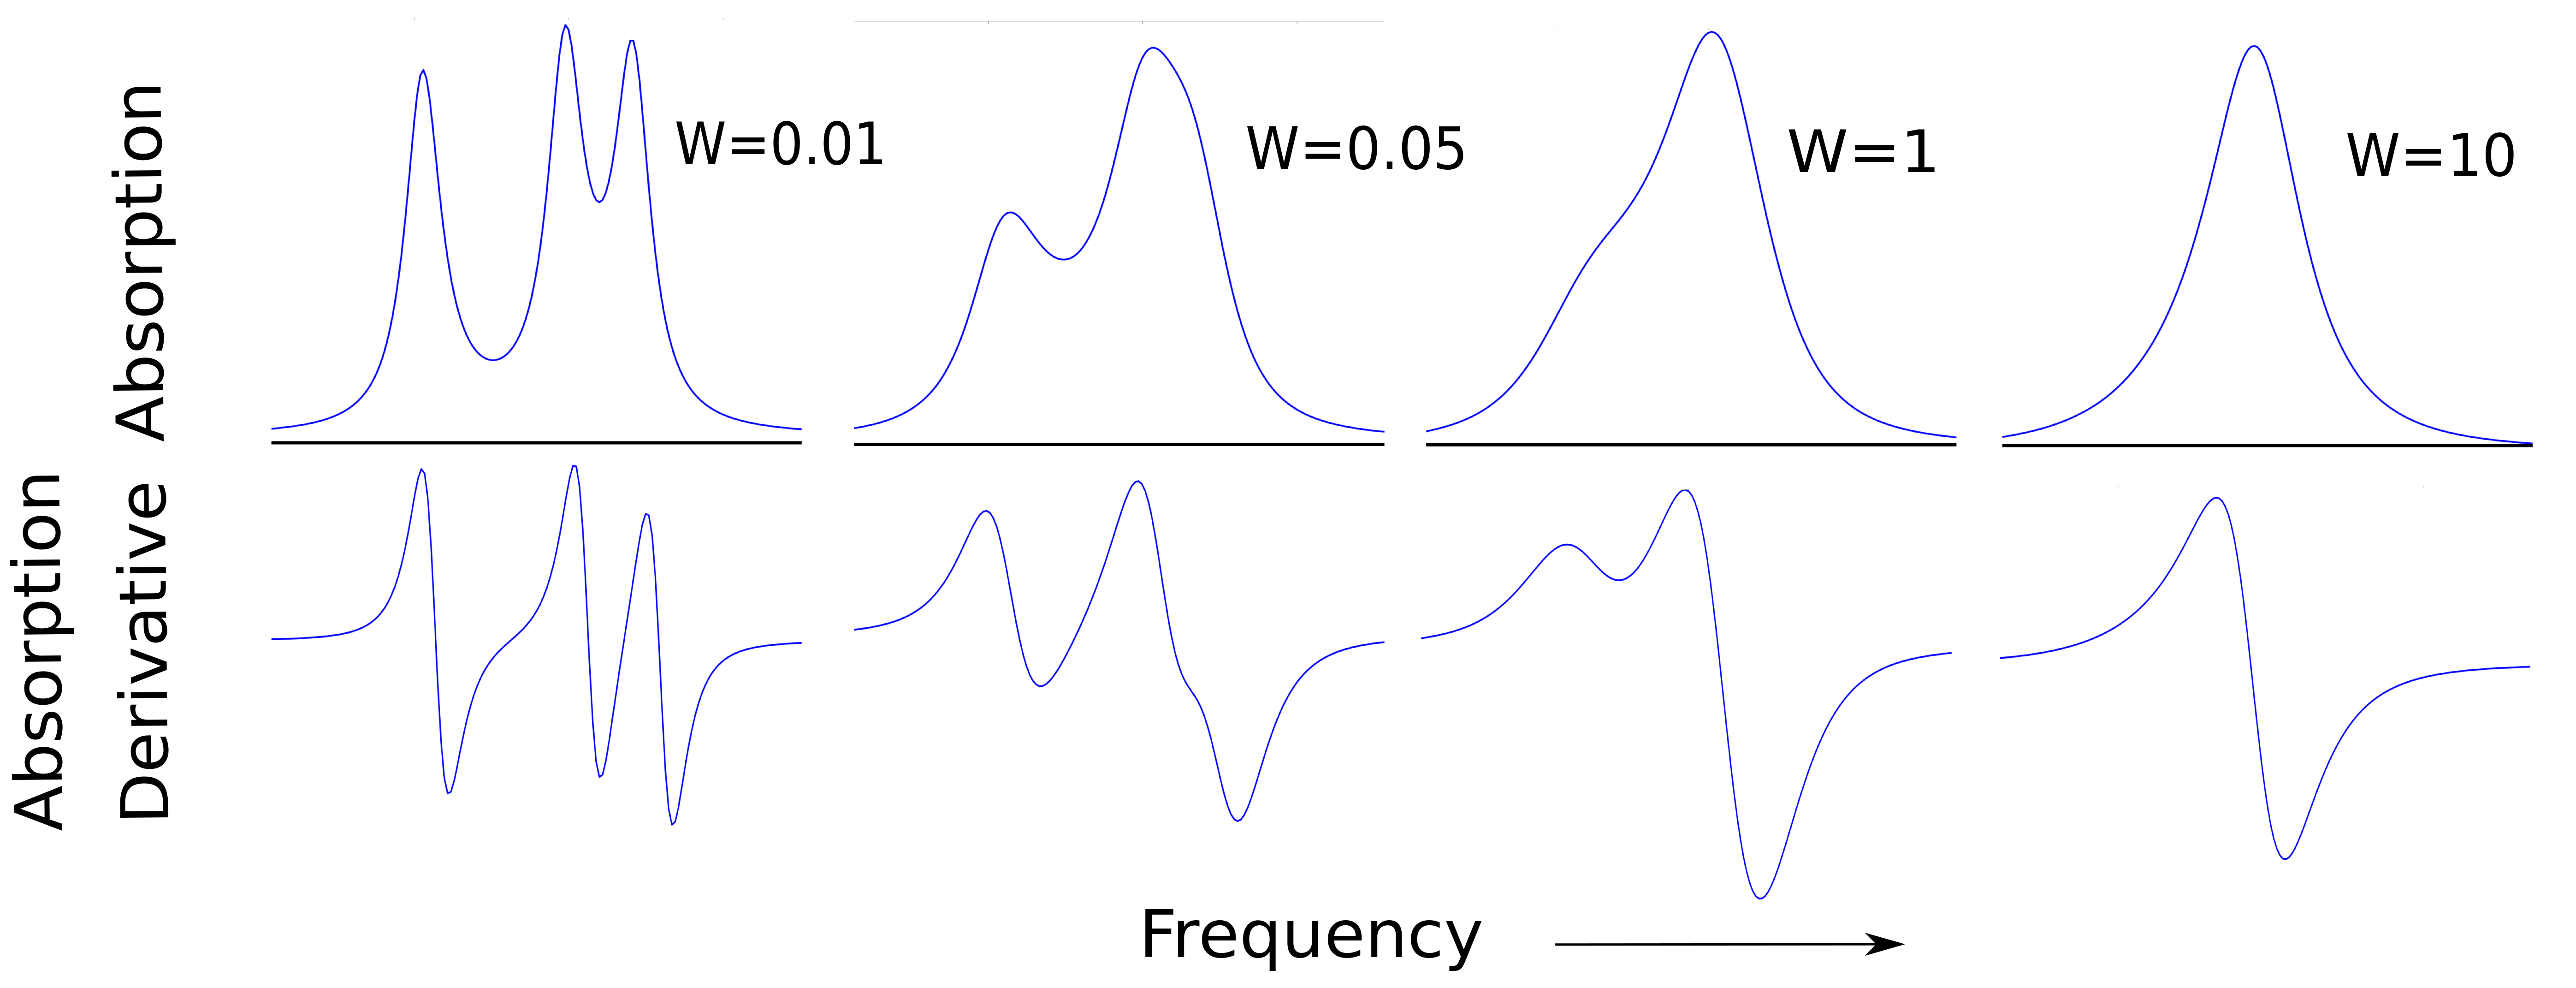
\includegraphics[height=8cm,width=1\textwidth]{figures/chap2/gtenanisat1.png}
\caption{Evolution of NMR line shapes with increase of transition rates $W$ for $I=1/2$ nucleus in a fixed magnetic field along $z$ axis and fluctuating local magnetic fields $h$ along (a) $x$ axis, (b) $y$ axis and (c) $z$ axis. Simulated using AI alagorithm}
\label{figure:gten1}
\end{figure}
There are no significant differences between 6 and 48 stochastic brining computational relief to us. 
\begin{figure}[h!]
\centering
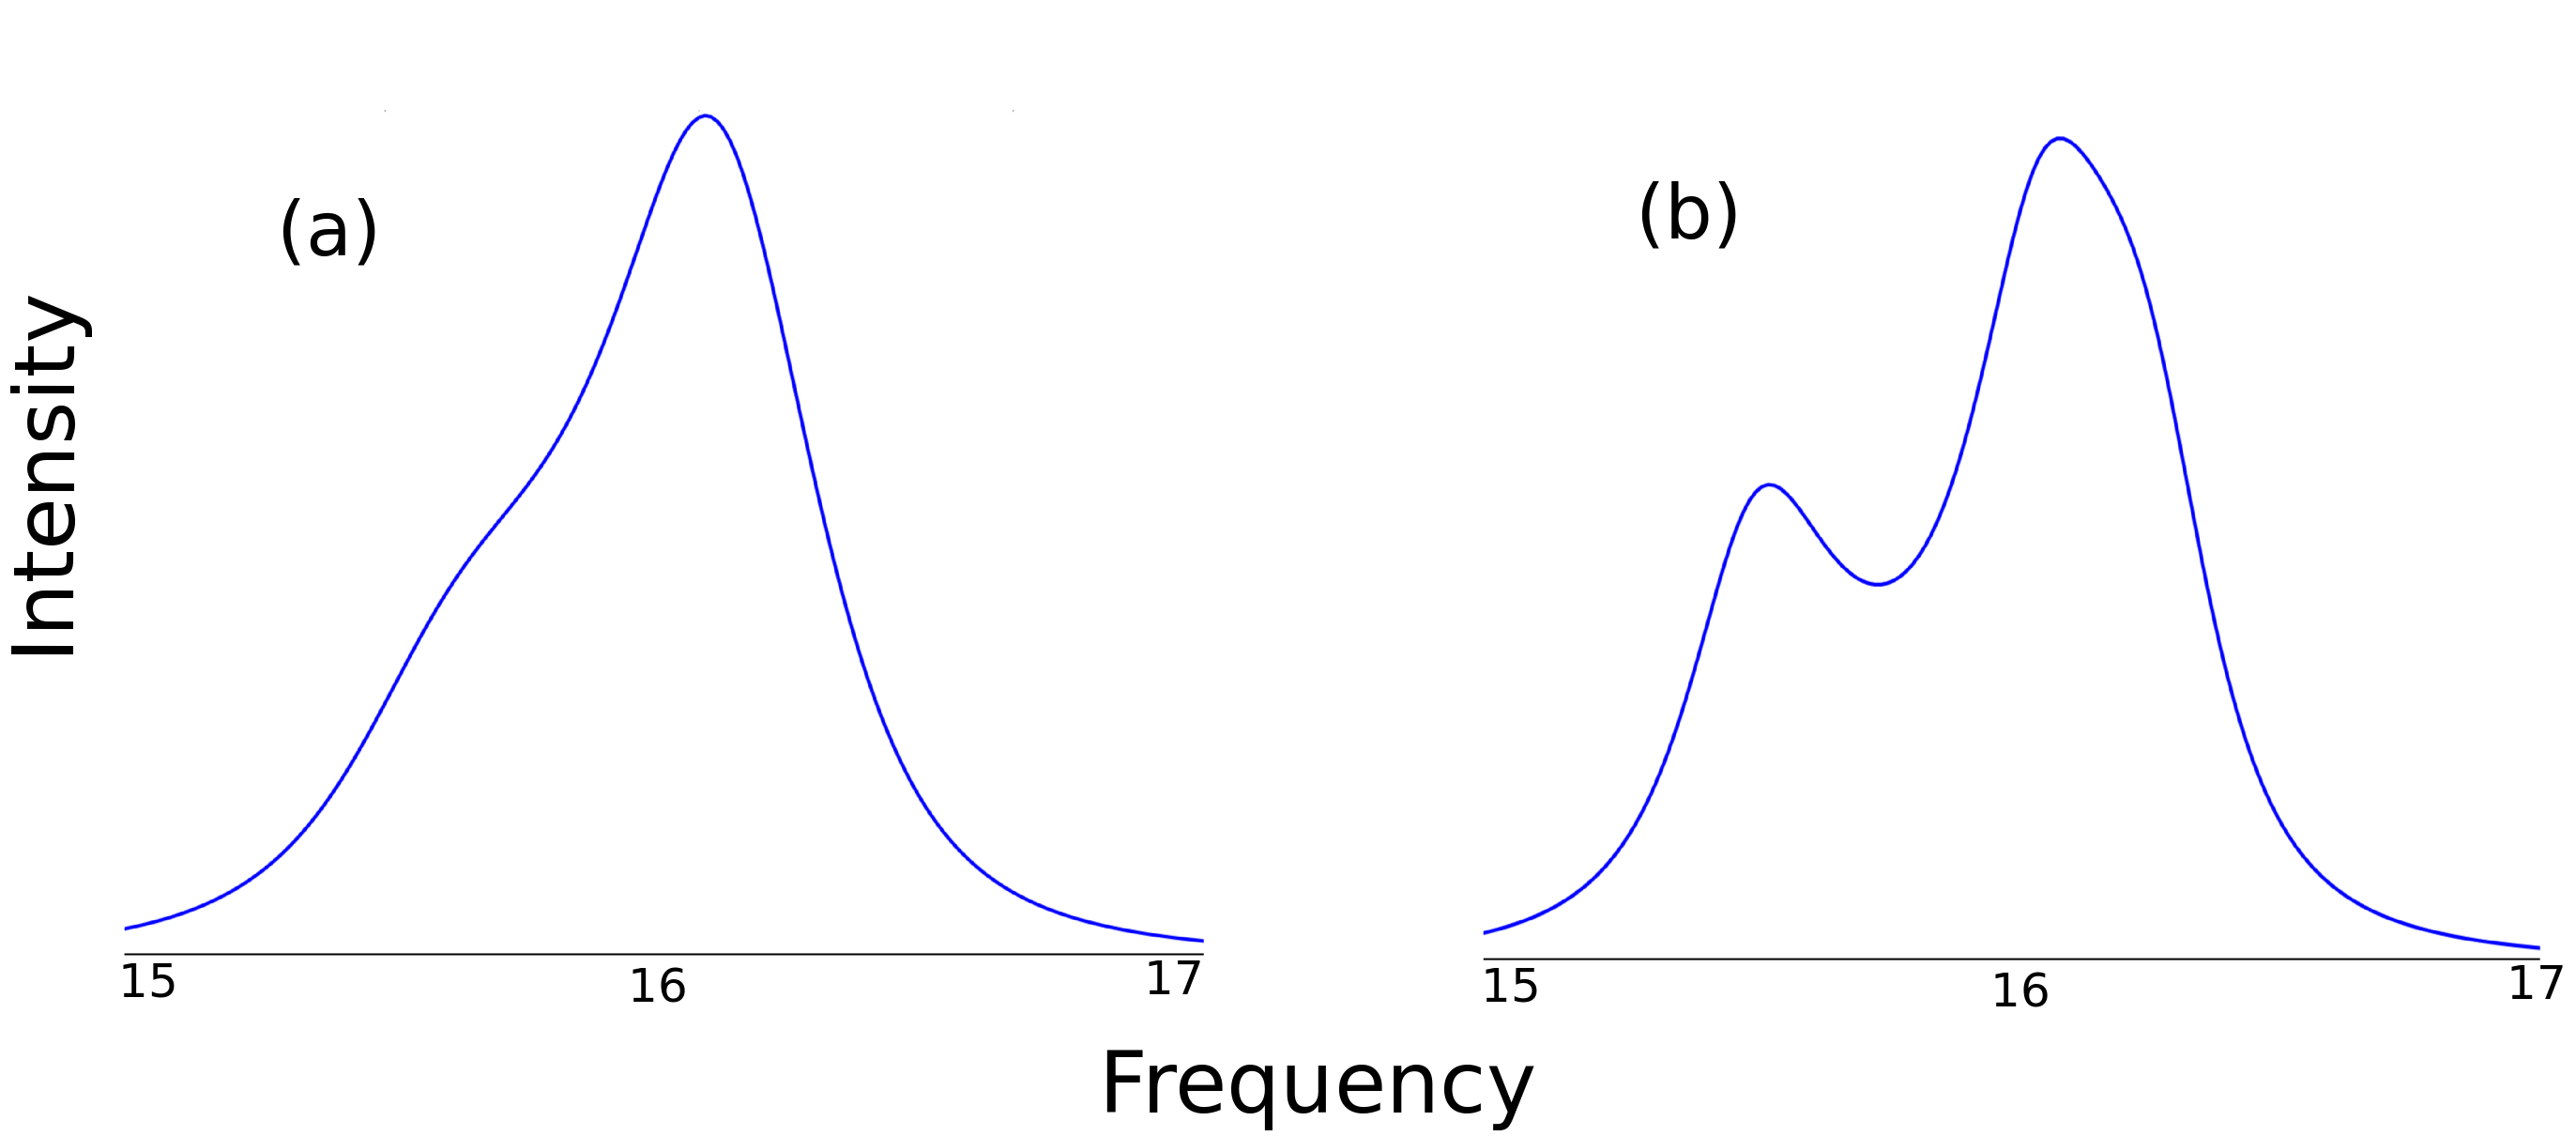
\includegraphics[height=8cm,width=1\textwidth]{figures/chap2/gtenanisat2.png}
\caption{Evolution of NMR line shapes with increase of transition rates $W$ for $I=1/2$ nucleus in a fixed magnetic field along $z$ axis and fluctuating local magnetic fields $h$ along (a) $x$ axis, (b) $y$ axis and (c) $z$ axis. Simulated using AI alagorithm}
Interestingly that using unequal a priori probability between states transition and using transition rates matrix designed in Eq.\ref{eq:Wmat2} setting $s=0.1,m=1$ and $f=100$ line shape tend to represent the case of axial symmetry or that $g_{xx}=g_{yy}<g_{zz}$ 
\label{figure:gterates}
\end{figure}
\clearpage
\subsection{Modelling Coupled Spins}\label{coupledspinsection}
The more complicated and fascinating interest for our group occurs when unpaired electron spin is interacting with nuclei. Thus a hyperfine interaction should be added. But first lets modify Eq.\ref{eq:37} adding additional sets of bra and kets for the unpaired electron quantum states $\langle m_{0s},m_{1s},S_0,S_1|$ and $|S_0,S_1,m_{0s}',m_{1s}'\rangle$ on both sides.  
\begin{multline}\label{eq:newbras}
P(\omega)=
\frac{2}{\Gamma(2I_0+1)}\mathcal{H}^{(-)}\delta_{m_{1I}m_{0I}}\delta_{m_{1S}m_{0S}}\mathcal{H}^{(+)}\delta_{m_{1I}'m_{0I}'}\delta_{m_{1S}'m_{0S}'} \\ \times[s\delta_{ab}\delta_{m_{1I}m_{1I}'}\delta_{m_{0I}m_{0I}'}\delta_{m_{1S}m_{1S}'}\delta_{m_{0S}m_{0S}'}-(a|W|b)\delta_{m_{0I}m_{0I}'}\delta_{m_{1I}m_{1I}'}\delta_{m_{0S}m_{0S}'}\delta_{m_{1S}m_{1S}'} \\ -i(a|F|a)\delta_{ab}[\langle I_0S_0m_{0I}m_{0S}|V_j|I_0S_0m_{0I}'m_{0S}'\rangle \delta_{m_{0I}m_{0I}'}\delta_{m_{0S}m_{0S}'}\\-\langle I_1S_1m_{1I}m_{1S}|V_j|I_1S_1m_{1I}'m_{1S}\rangle\delta_{m_{1I}m_{1I}'}\delta_{m_{1S}m_{1S}'}]^{-1}
\end{multline} 
Starting vectors $\mathcal{H}^{(+)}$ and $\mathcal{H}^{(-)}$ that define proper electronic magnetization components for the line shape are modified accordingly to \cite{bmr}: 
\begin{equation}
\langle \mathcal{H}^{(+)} \rangle=\langle S_x\otimes I_1 \rangle
\end{equation}
Where $I_1$ is a unit operator in nuclear spin space. $\langle S_x\rangle$ can be easily found in terms of rising and lowering operators and corresponding matrix constructed. \\*
Similarly to the ISTO transformation of the Zeeman part of Hamiltonian it is possible to write all components of the transformed hyperfine interaction term. Starting with spin operators in laboratory frame:   
\begin{subequations}\label{eq:hyperA}
\begin{align}
A^{[2],L}_{\pm2,(hf)} & =-\frac{1}{2}S_{\pm}I_{\pm}\\
A^{[2],L}_{\pm1,(hf)} & =\pm\frac{1}{2}(S_{\pm}I_{z}+S_zI_{\pm})\\
A^{[2],L}_{0,(hf)} & =-\sqrt{\frac{2}{3}}\big(S_{z}I_{z}-\frac{1}{4}(S_+I_-+S_-I_+)\big)\\
A^{[0],L}_{0,(hf)} & =\frac{1}{\sqrt{3}}\big(S_{z}I_{z}+\frac{1}{2}(S_+I_-+S_-I_+)\big)
\end{align}
\end{subequations}
Correspondingly principal components of the $A$-tensor: 
\begin{subequations}\label{eq:HyperAA}
\begin{align}
F^{[2],P}_{\pm2,(hf)} & =-\frac{1}{2}\beta_e(A_{xx}-A_{yy})\\
F^{[2],P}_{\pm1,(hf)} & =0\\
F^{[2],P}_{0,(hf)} & =-\sqrt{\frac{2}{3}}\beta_e\big(A_{zz}-\frac{1}{2}(A_{xx}+A_{yy})\big)\\
F^{[0],P}_{0,(hf)} & = \frac{1}{\sqrt{3}}\beta_e(A_{xx}+A_{yy}+A_{zz})
\end{align}
\end{subequations}
Transformation between laboratory and principal axis system for the hyperfine interaction can be done in similar fashion as for the $g$ tensor. Working in the linear response regime only commuting terms with the Zeeman Hamiltonian are of interest or in other words terms that are proportional to $S_z$. Effective Hamiltonian for Hyperfine part only can be written thus as: 
\begin{equation}
\mathcal{H}_{eff}'=A_{0,(hf)}^{[0]}F_{0,(hf)}^{[0]}+A_{0,(hf)}^{[2]} F_{0,(hf)}^{[2]}+A_{+1,(hf)}^{[2]} F_{+1,(hf)}^{[2]}+A_{-1,(hf)}^{[2]} F_{-1,(hf)}^{[2]}
\end{equation}
\begin{equation}
\mathcal{H}_{eff}'=(\frac{1}{\sqrt{3}})S_zI_zF_{0,(hf)}^{[0]}+(-\sqrt{\frac{2}{3}})S_zI_zF_{0,(hf)}^{[2]}+\frac{1}{2}S_zI_- F_{+1,(hf)}^{[2]}+(\frac{1}{2})S_zI_+ F_{-1,(hf)}^{[2]}
\end{equation}
The only interest brings the terms that a partially commute with the Zeeman interaction namely that are proportional to $I_z$ operators coupled with $S_z$ or in other words $S_zI_z$. In this way only similar to Zeeman term quantum states are coupled. In the case when hyperfine interaction is strong compared to Zeeman it is important to include a spin "flipping" terms that do not change electronic spin states or terms that are $S_zI_{\pm}$. This terms do not commute with the Zeeman Hamiltonian and they induce additional transition between the sates in the system known as "Pseudosecular". Thus we have approached Blume~\cite{blume} model with the general form of the Hamiltonian. As usual "Nonsecular" terms have been dropped of namely $A_{\pm2,(hf)}^{[2]}$. Now total Hamiltonian assuming that principal component of the Zeeman $g$ tensor and Hyperfine $A$ tensor are coincide so that there are no mutual difference between rotational transformation of their principal components can be written,
\begin{multline}
\mathcal{H}_{total}=H_{eff}+H_{eff}'=\frac{1}{\sqrt{3}}F_{0}^{[0]}(S_zI_z+S_zB_z) \\ +(-\sqrt{\frac{2}{3}})F_{0}^{[2]}(S_zB_z+S_zI_z)+\frac{1}{2}S_zI_- F_{+1}^{[2]} +(\frac{1}{2})S_zI_+ F_{-1}^{[2]}
\end{multline}
\subsubsection{Coupled Spins 1/2 to 1/2}\label{coupledspinonehalfsection}
To start out with lets consider $S=1/2$ and $I=1/2$ case. Allowed transitions are obvious for the Zeeman interaction and overlapping Hyperfine are defined with the kronecker deltas and more interesting are the two allowed transitions for the "pseudosecular" part of the Hamiltonian:
$$|m_S=-1/2,m_I=1/2\rangle\rightarrow|m_S=1/2,m_I=1/2\rangle$$ 
and 
$$|m_S=-1/2,m_I=-1/2\rangle\rightarrow|m_S=1/2,m_I=-1/2\rangle$$ 
On the Fig.\ref{figure:spin05} result is given including only terms that are commuting with the Zeeman Hamiltonian. 
\begin{figure}[h!]
\centering
\includegraphics[width=1\textwidth]{figures/chap2/gtenanisatotal.eps}
\caption{Evolution of NMR line shapes with increase of transition rates $W$ for $I=1/2$ nucleus in a fixed magnetic field along $z$ axis and fluctuating local magnetic fields $h$ along (a) $x$ axis, (b) $y$ axis and (c) $z$ axis. Simulated using AI alagorithm}
\label{figure:spin05}
\end{figure}
\subsubsection{Spins 1 to 1/2}\label{coupledspinonesection}
Similarly we can model $S=1$ to $I=1/2$ coupling. 
\begin{figure}[h!]
\centering
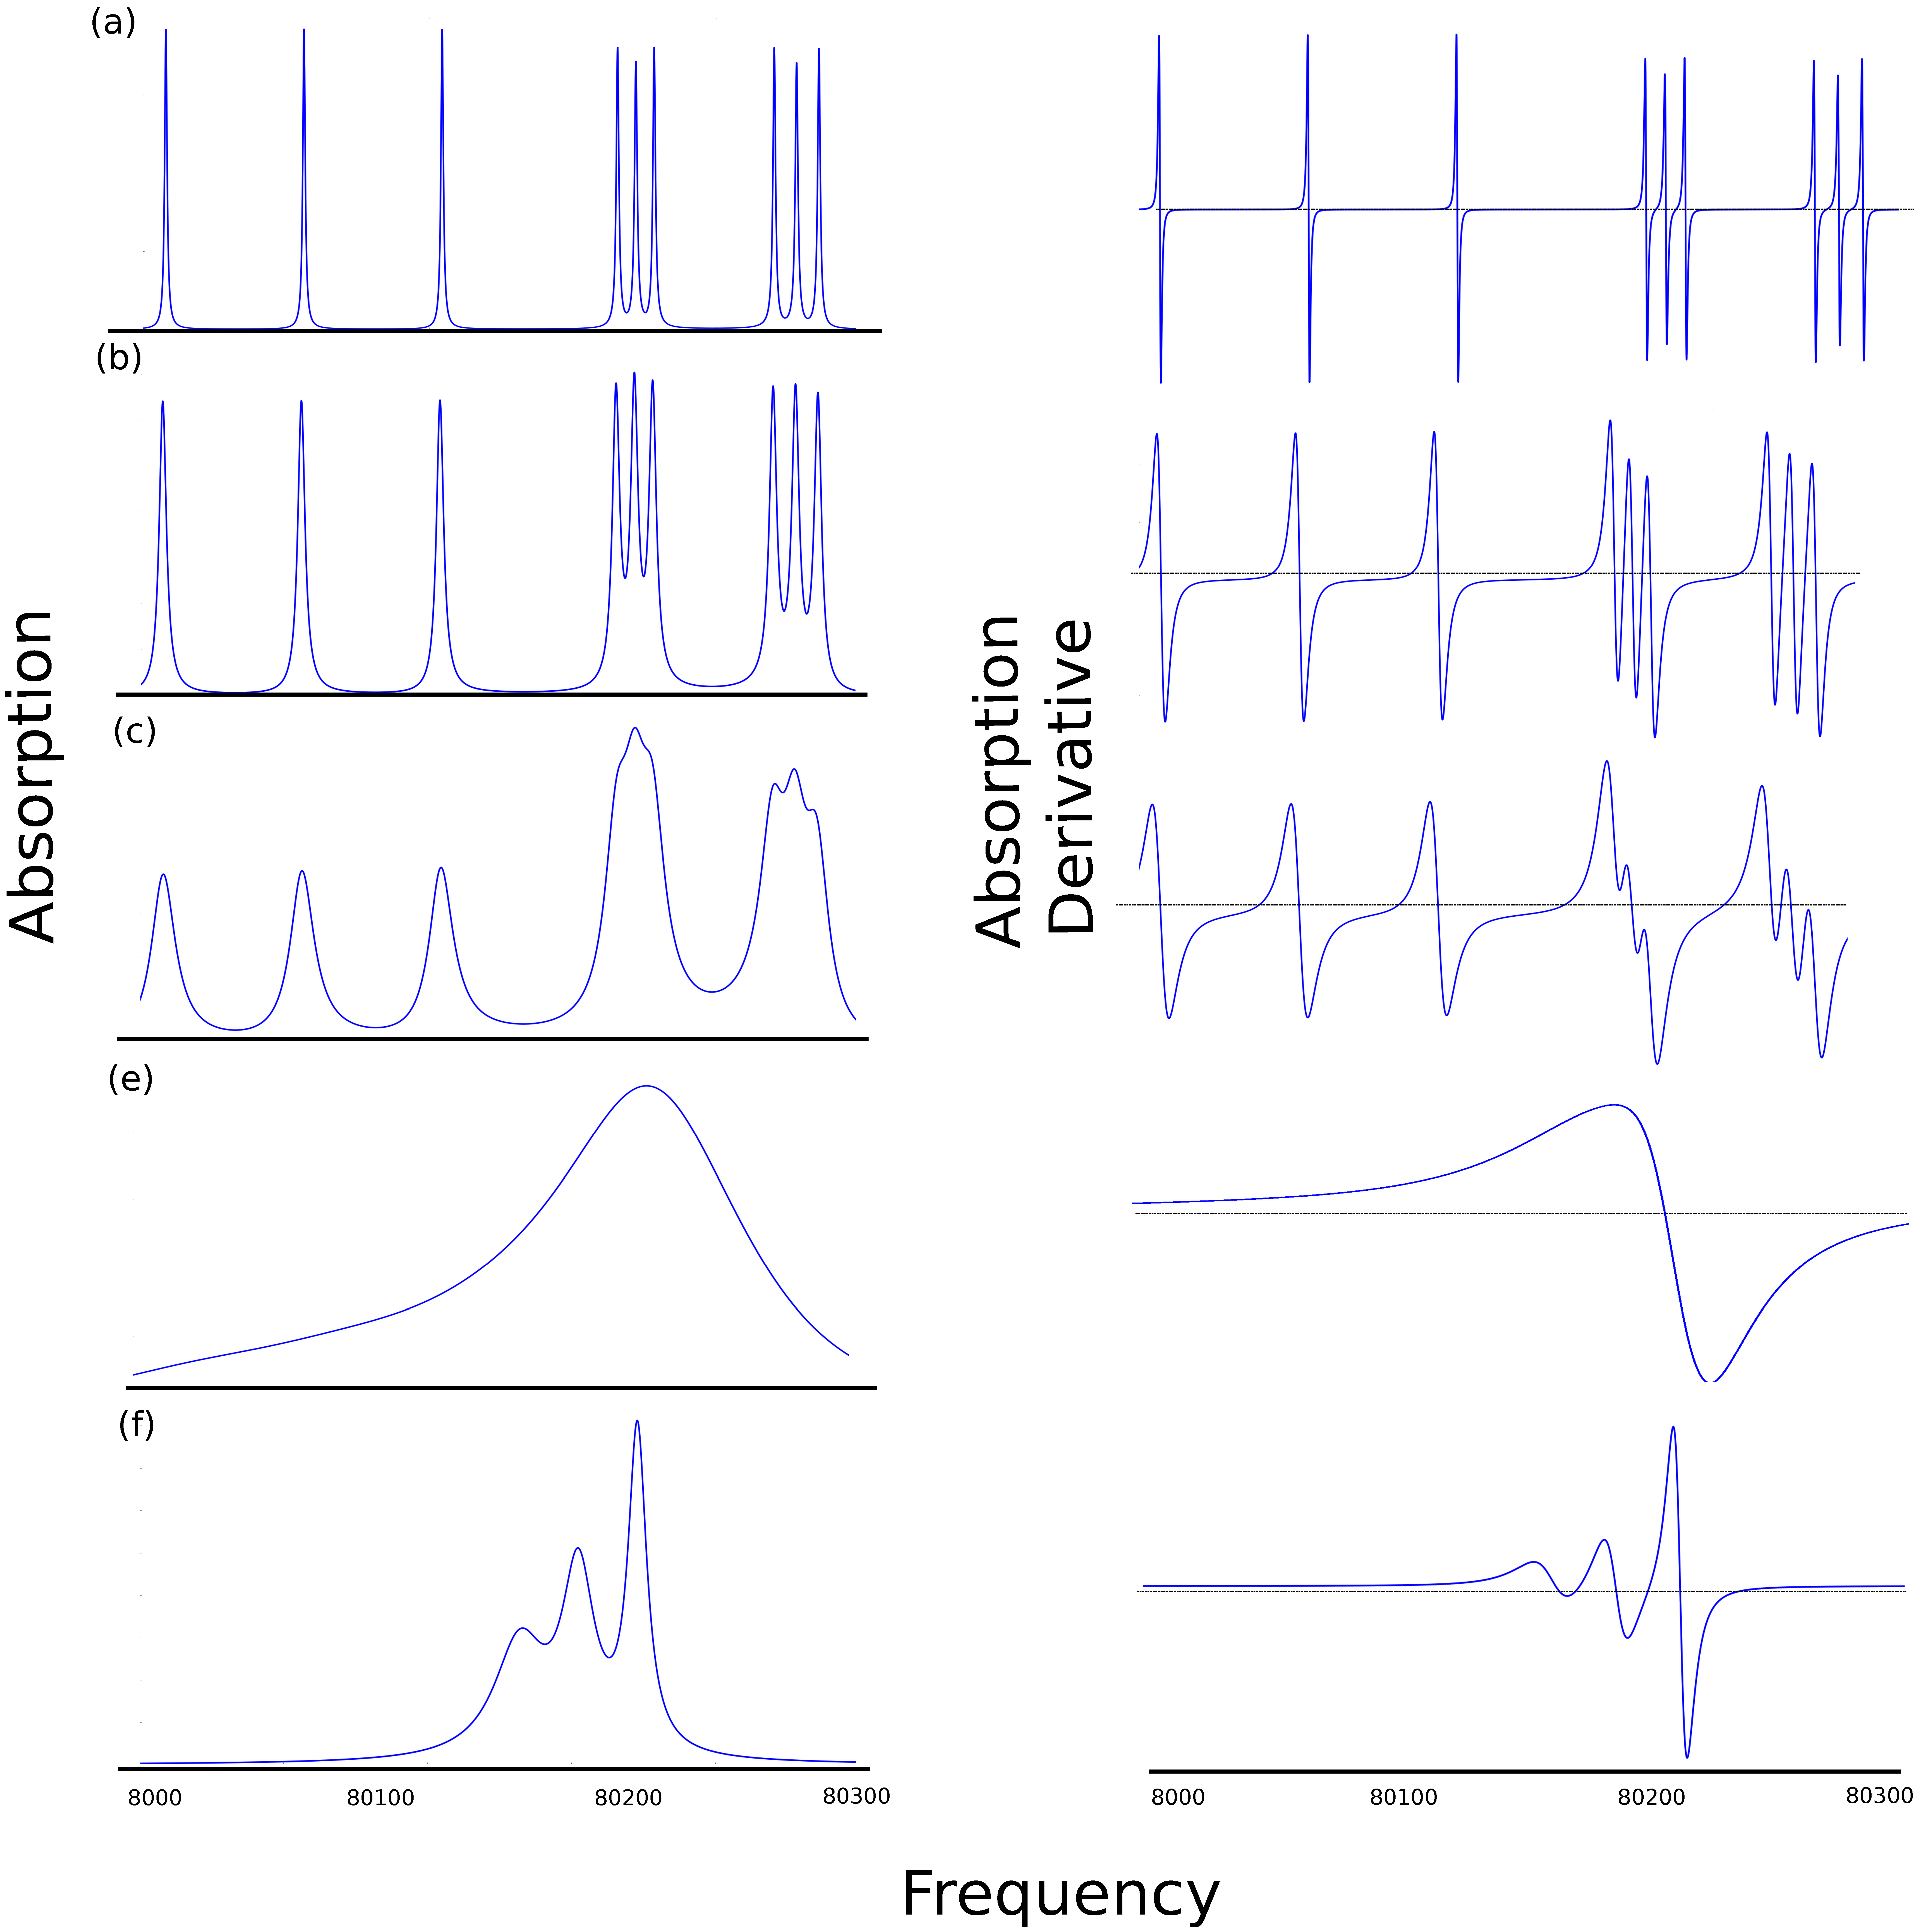
\includegraphics[width=1\textwidth]{figures/chap2/spinone.eps}
\caption{Evolution of NMR line shapes with increase of transition rates $W$ for $I=1/2$ nucleus in a fixed magnetic field along $z$ axis and fluctuating local magnetic fields $h$ along (a) $x$ axis, (b) $y$ axis and (c) $z$ axis. Simulated using AI alagorithm for 6 states}
\label{figure:spin05der}
\end{figure}
\begin{figure}[h!]
\centering
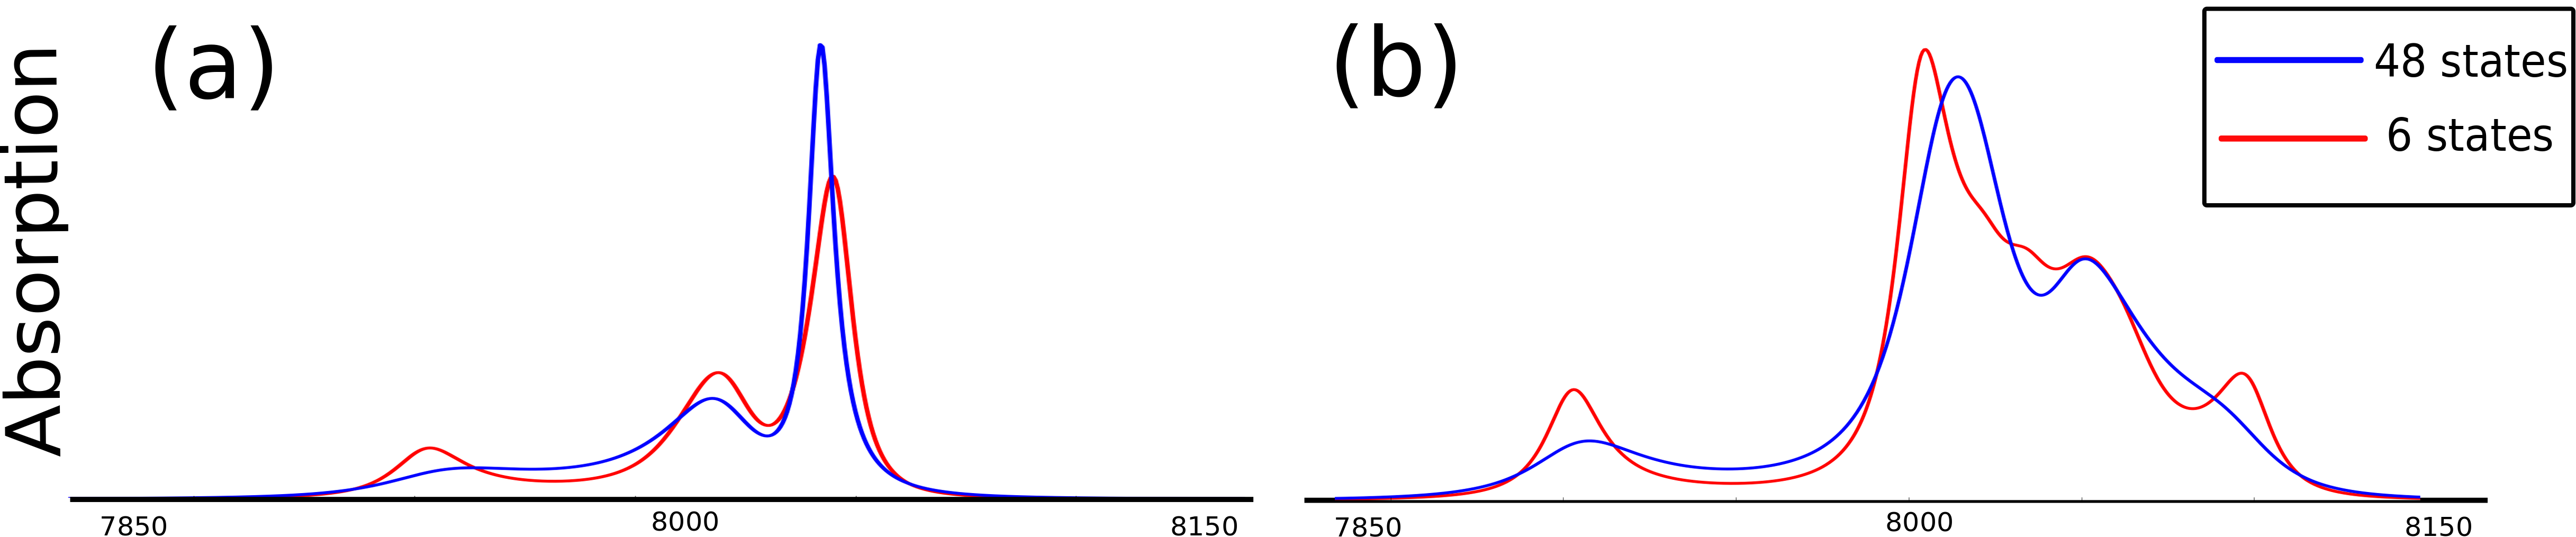
\includegraphics[width=1\textwidth]{figures/chap2/spin051moderate.png}
\caption{Computed high field EPR spectra for $^{14}N$ (5a) and $^{15}N$ (5b) nitroxide spin-labels arising from 6(blue line) and 48(red line) state models in medium transition rate regime. Transition rate W=5.}
\label{figure:spin05der1}
\end{figure}
\subsection{Quadrupolar Interaction}
\begin{figure}[h!]
\centering
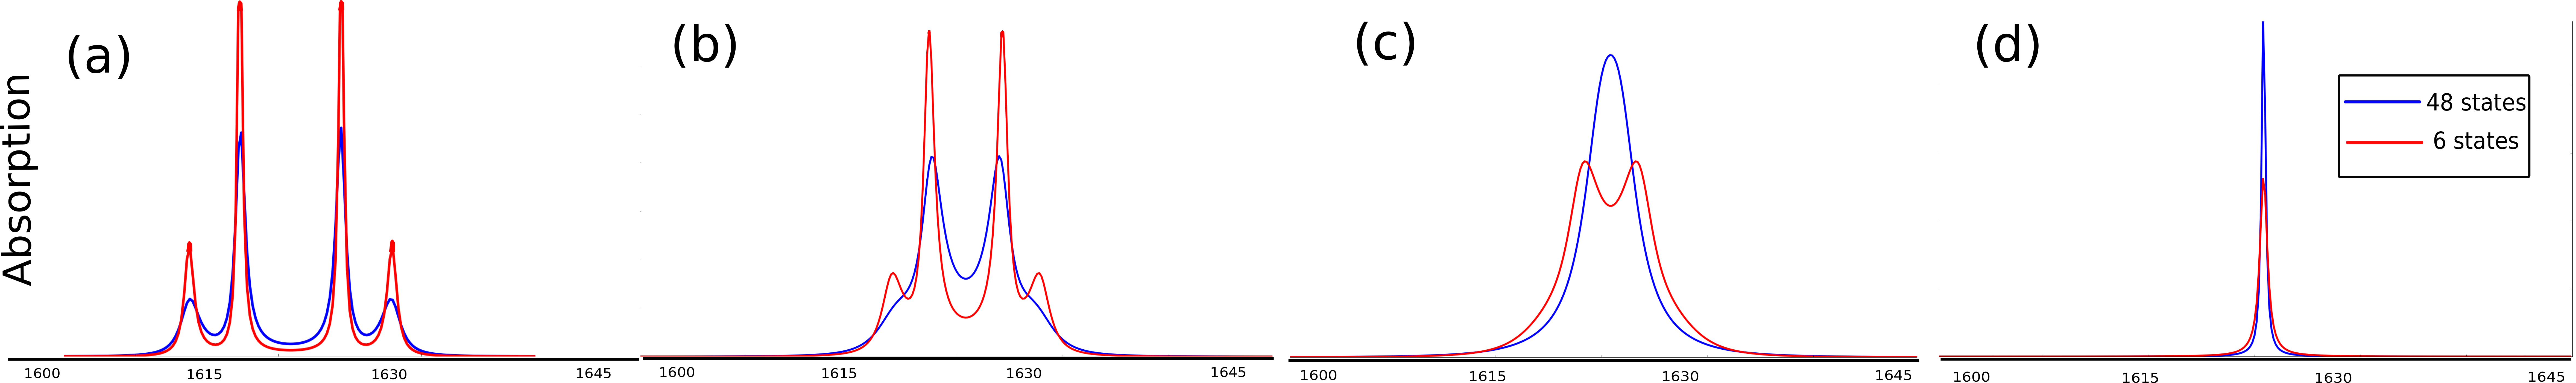
\includegraphics[width=1\textwidth]{figures/chap2/2site_final.png}
\caption{Computed high field EPR spectra arising from the isotropic stochastic modulation of the quadrupole moment of an $^{14}N$ nucleus contained within the nitroxide spin label. The red line is the spectrum arising from the 6 state model. The blue line is the simulation arising from 48 state model. Transition rates are (a)W=0.1,(b) W=0.3,(c)W=1 and (d)W=10}
\label{figure:spin05der2}
\end{figure}
\subsection{Conclusion}
\clearpage